\documentclass[11pt]{article}
\usepackage[margin=1in]{geometry}
\usepackage{amsmath}
\usepackage{graphicx}
\usepackage{booktabs}
\usepackage{parskip}

\begin{document}

\begin{center}
{\Large\bfseries Macro HW1}\\[0.35em]
{\small Xingming Li \quad School ID: 1432037}
\end{center}

\hrule
\medskip

\textbf{Question 1.} Every entry is a percent deviation from trend.

\begin{center}
\begin{tabular}{lcc}
\toprule
Variable & \% Standard Deviation & Correlation with Output \\
\midrule
Output                         & 1.70 & 1.00 \\
Consumption                    & 1.60 & 0.81 \\
Investment                     & 6.45 & 0.63 \\
Gov't Consumption Expenditure  & 1.01 & 0.22 \\
Gov't Investment Expenditure   & 3.20 & $-0.06$ \\
Exports                        & 3.70 & 0.76 \\
Imports                        & 4.72 & 0.82 \\
Net Exports                    & 0.69 & $-0.30$ \\
Hours Worked                   & 2.16 & 0.89 \\
Labour Productivity            & 1.01 & $-0.23$ \\
Capital                        & 0.87 & $-0.15$ \\
Capital Productivity           & 2.02 & 0.90 \\
Nominal Exchange Rate          & 3.86 & $-0.12$ \\
Price                          & 1.32 & 0.25 \\
\bottomrule
\end{tabular}
\end{center}

\begin{center}
$\operatorname{corr}(\text{hours worked},\ \text{labour productivity}) = -0.65$
\end{center}

\bigskip
\textbf{Question 2.}

\textbf{(a)}

\begin{center}
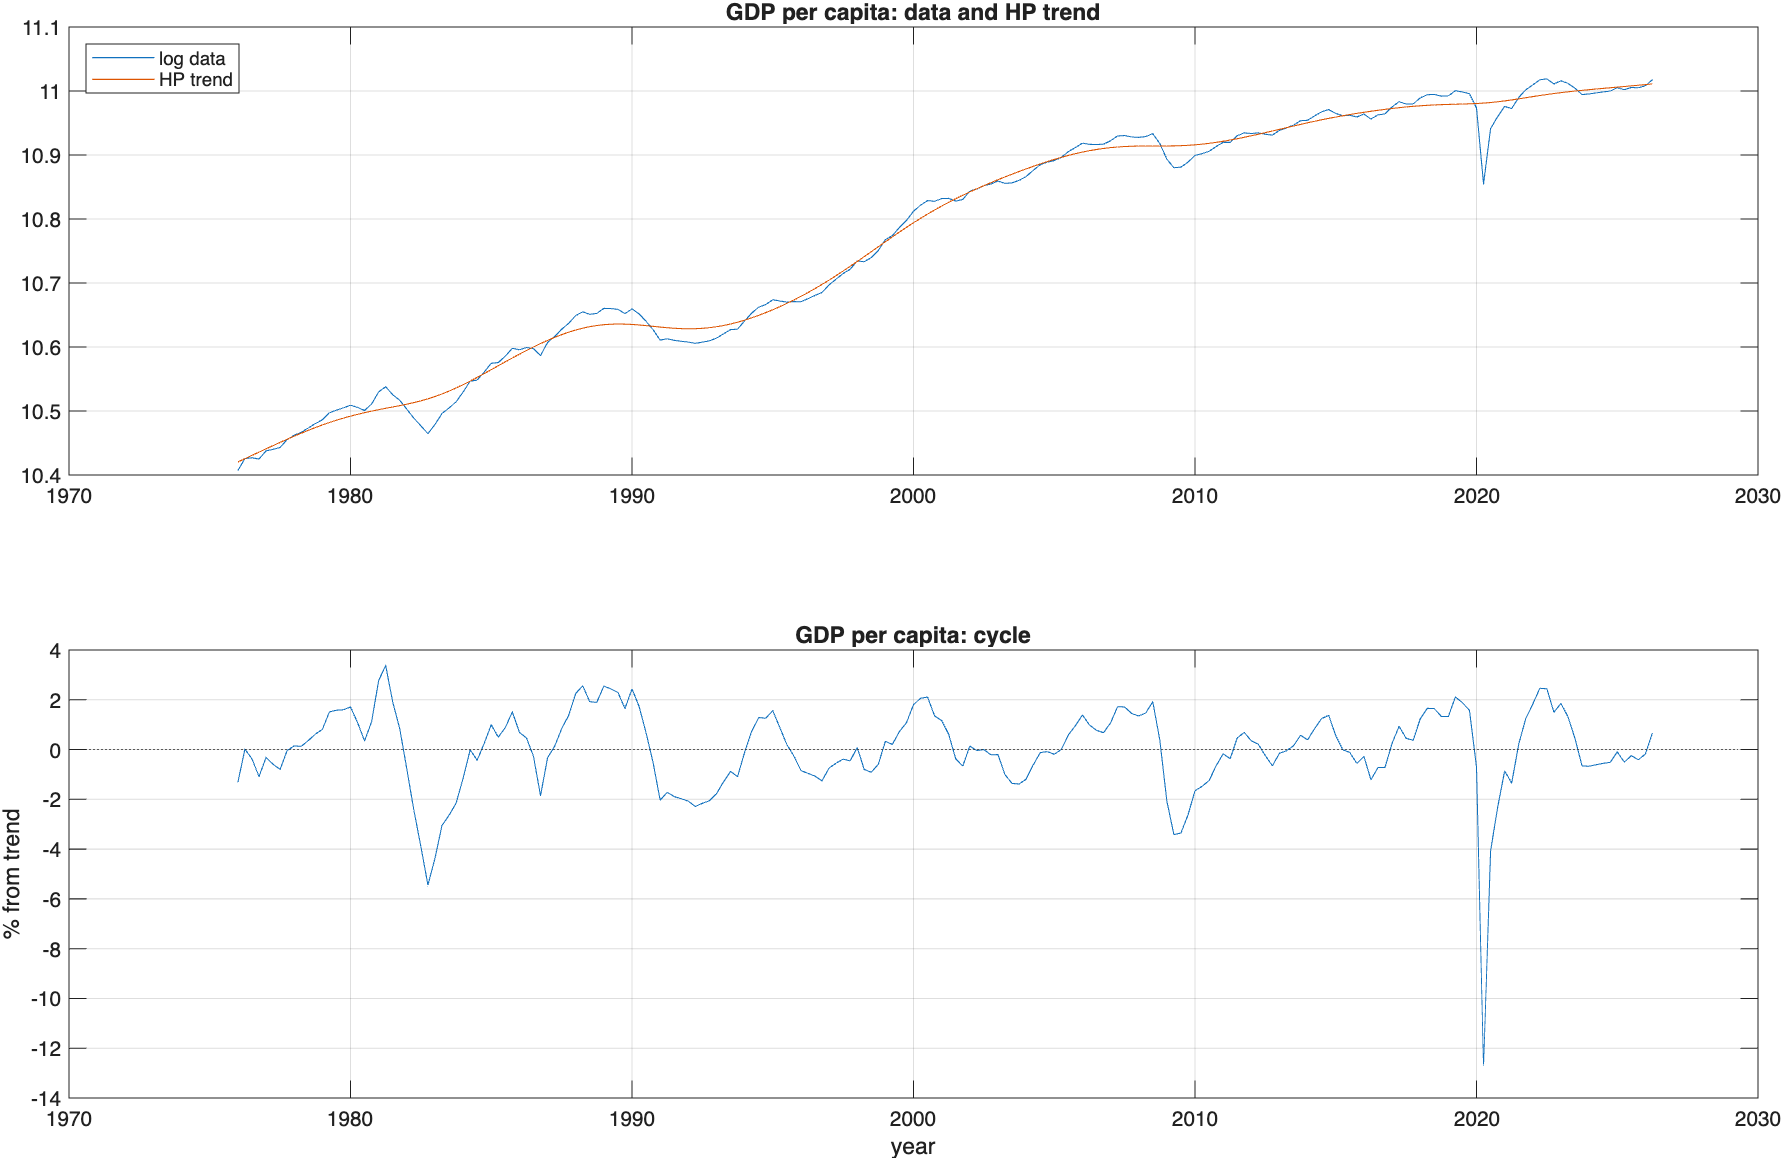
\includegraphics[width=0.70\textwidth]{q2_gdp.png}\\[0.4em]
{\small Figure 1. GDP per capita: data and HP trend (top), cycle (bottom).}
\end{center}

\begin{center}
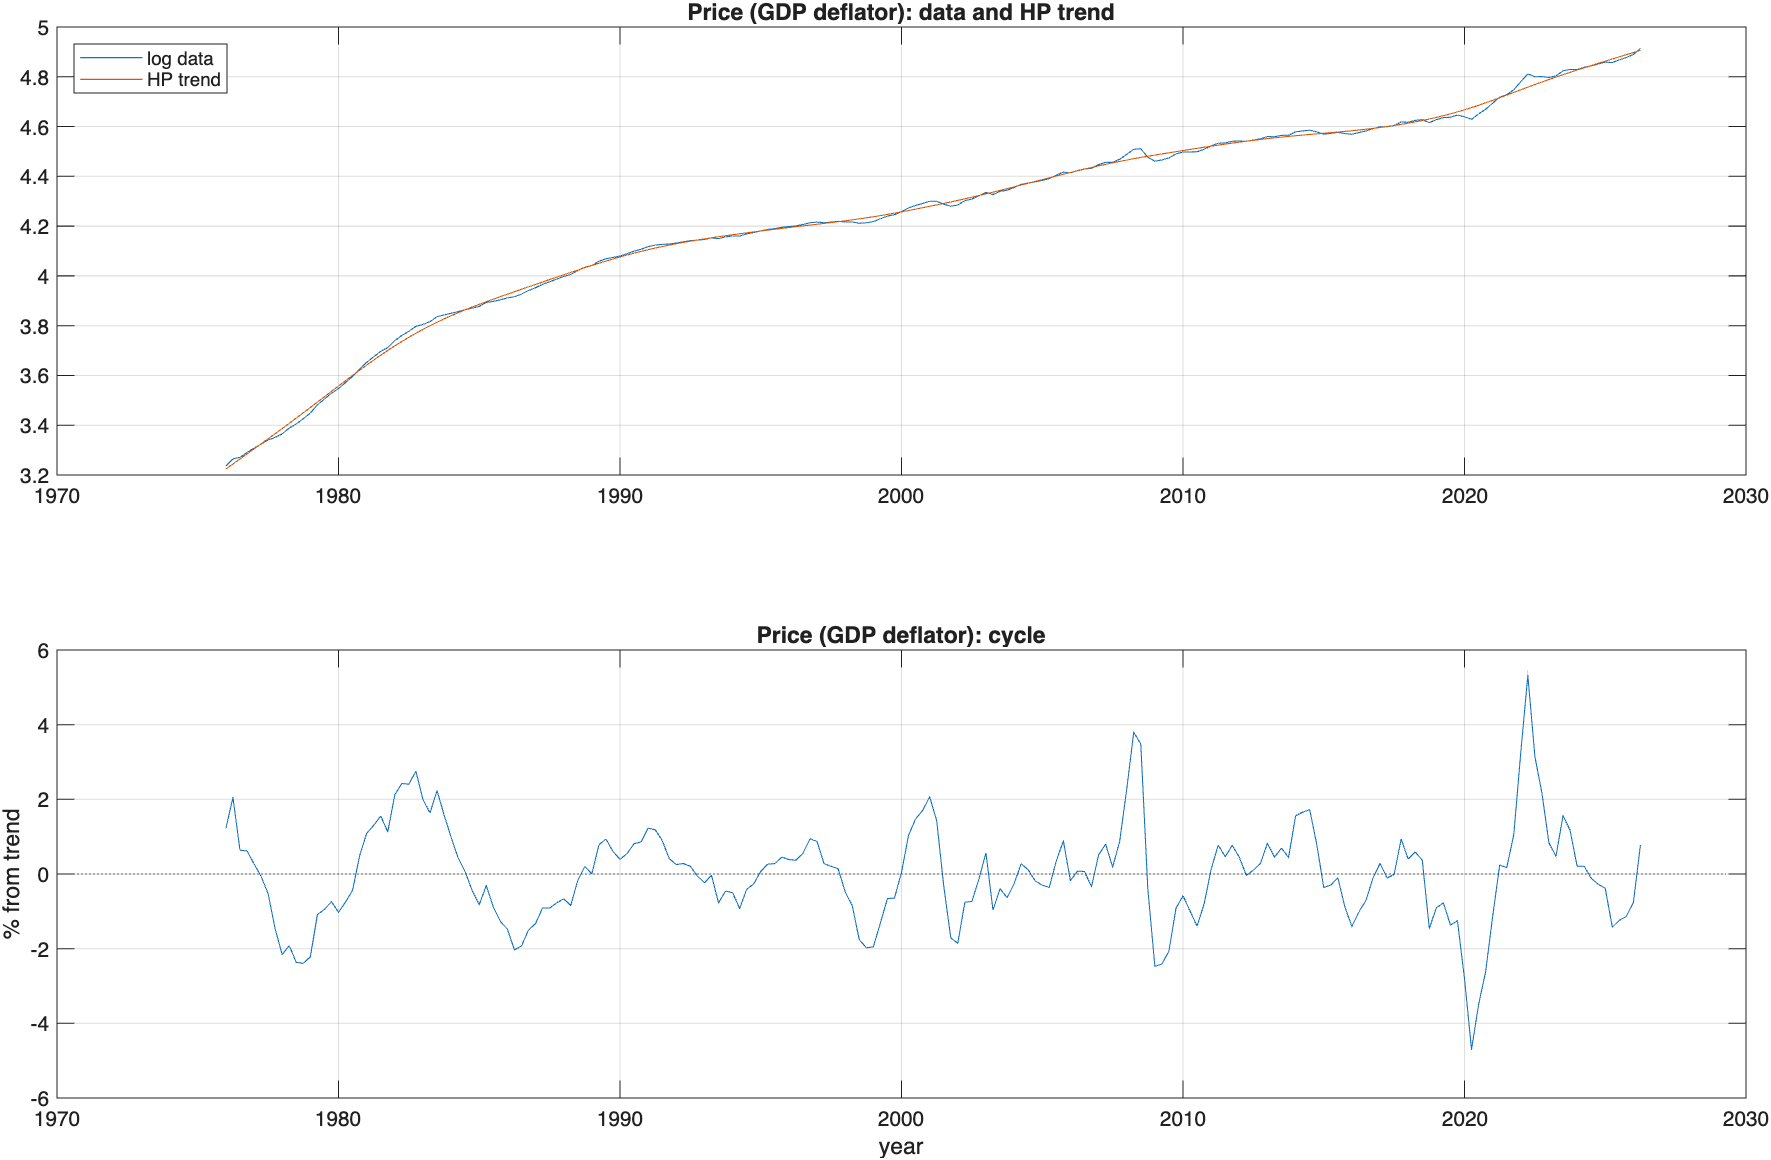
\includegraphics[width=0.70\textwidth]{q2_price.png}\\[0.4em]
{\small Figure 2. Price (GDP deflator): data and HP trend (top), cycle (bottom).}
\end{center}

\textbf{(b)} GDP per capita peaks in 2008Q3, so that is where the recession starts. Output
falls for three quarters, drops below trend in 2009Q1 and bottoms in 2009Q2. The recovery
starts there, and output is back at trend in 2011Q3.

\textbf{(c)}

\begin{center}
\begin{tabular}{lcccc}
\toprule
Episode & Peak & Trough & Depth (\%) & Duration (quarters) \\
\midrule
Early 1980s     & 1981Q2 & 1982Q4 & $-5.44$ & 6  \\
Early 1990s     & 1989Q1 & 1992Q2 & $-2.29$ & 13 \\
Great Recession & 2008Q3 & 2009Q2 & $-3.42$ & 3  \\
\bottomrule
\end{tabular}
\end{center}

Depth is the lowest point of the cycle and duration runs peak to trough. The Great Recession
was about 1.5 times as deep as the early 1990s, roughly 60\% as deep as the early 1980s, and
at three quarters the shortest of the three. The early 1990s was the slowest: output stayed
below trend for 14 quarters, against 11 in the early 1980s and 10 in the Great Recession.

{\small The 1990s start is a close call. The cycle also peaks at 1988Q2 ($+2.56\%$), a hair
above 1989Q1 ($+2.55\%$). I use 1989Q1 because it starts the sustained decline; counting from
1988Q2 would make the episode 16 quarters instead of 13.}

\bigskip
\textbf{Question 3.} A collapse in demand. Output and prices fell together over
2007Q1--2011Q4 (correlation $+0.83$), with the price cycle bottoming at $-2.5\%$ in 2009Q1
and output at $-3.4\%$ in 2009Q2. A supply shock would have pulled the two apart: over
1979Q1--1983Q4, the oil-shock years, the correlation is $-0.61$, with output 5.4\% below
trend while prices ran 2.8\% above it. The collapse itself came from the financial crisis:
credit tightened, households lost wealth, firms cut investment, and U.S. demand for Canadian
exports fell.

\bigskip
\textbf{Question 4.}

\begin{center}
\begin{tabular}{lccc}
\toprule
Variable & Fall, 2019Q4--2020Q2 & Cycle low & Back at 2019Q4 level \\
\midrule
Output (GDP p.c.) & $-13.1\%$ & $-12.6\%$ (2020Q2) & 2021Q4 \\
Price (deflator)  & $-1.7\%$  & $-4.7\%$ (2020Q2)  & 2020Q3 \\
Hours worked      & $-21.9\%$ & $-21.9\%$ (2020Q2) & 2023Q1 \\
\bottomrule
\end{tabular}
\end{center}

The falls are percent changes in the population-deflated level from 2019Q4 to 2020Q2. Output
dropped 13.1\%, and the trough was 3.7 times deeper than the Great Recession's, but output
was back at its pre-pandemic level by 2021Q4. Hours fell 21.9\%, so output per hour rose, and
hours were the last to recover, not until 2023Q1. Prices dipped only 1.7\%.

\end{document}
